\documentclass{article}
\usepackage[utf8]{inputenc}
\usepackage{indentfirst}
\usepackage{listings}
\usepackage{color}
\usepackage{graphicx}
\graphicspath{ {./img/} }
\definecolor{lightgray}{rgb}{.9,.9,.9}
\definecolor{darkgray}{rgb}{.4,.4,.4}
\definecolor{superdarkgray}{rgb}{.2,.2,.2}
\definecolor{purple}{rgb}{0.65, 0.12, 0.82}
\newcommand{\cit}[1]{{\fontfamily{qcr}\selectfont{\textcolor{superdarkgray}{#1}}}}
\newcommand{\bit}[1]{\textit{\textbf{#1}}}

% Taken from Lena Herrmann at 
% http://lenaherrmann.net/2010/05/20/javascript-syntax-highlighting-in-the-latex-listings-package
\lstdefinelanguage{JavaScript}{
  keywords={typeof, new, true, false, catch, function, return, null, catch, switch, var, if, in, while, do, else, case, break},
  keywordstyle=\color{blue}\bfseries,
  ndkeywords={class, export, boolean, throw, implements, import, this},
  ndkeywordstyle=\color{darkgray}\bfseries,
  identifierstyle=\color{black},
  sensitive=false,
  comment=[l]{//},
  morecomment=[s]{/*}{*/},
  commentstyle=\color{purple}\ttfamily,
  stringstyle=\color{red}\ttfamily,
  morestring=[b]',
  morestring=[b]"
}

\lstset{
   language=JavaScript,
   backgroundcolor=\color{lightgray},
   extendedchars=true,
   basicstyle=\footnotesize\ttfamily,
   showstringspaces=false,
   showspaces=false,
   numbers=left,
   numberstyle=\footnotesize,
   numbersep=9pt,
   tabsize=2,
   breaklines=true,
   showtabs=false,
   captionpos=b
}

\title{Async Tree Pattern}
\author{Guseyn Ismayylov}
\date{July 2018}

\begin{document}

\maketitle

\section{Introduction}

\textbf{Async Tree Pattern} is a declarative design pattern, the main purpose of which is to transform procedural code into the object-oriented(declarative) code in the asynchronous environment via async tree, which is the core idea of this pattern.

\section{Declarative vs Imperative}

The conception of the \textit{async tree} was created with assumption that declarative programming is much better than imperative style of writing code for big programs and systems. Declarative code is more readable, extensible and maintainable in general.

You may agree or disagree with this statement. It's only opinion of the author of this work.

Here it will be shown the difference between these two approaches by small example. Let's consider the following imperative code:  

\begin{lstlisting}

// Imperative, pseudocode
user = getUserFromDb(userId);
account = user.createNewAccount(accountInfo);
user.saveAccount(account);

\end{lstlisting}

It can be written in the declarative style:

\begin{lstlisting}

// Declarative, pseudocode
SavedAccount(
  CreatedAccount(
    UserFromDb(userId), accountInfo
  )
).call();

\end{lstlisting}

The example is quite small to demonstrate why declarative programming is preferable. Nevertheless, you can see that declarative code always shows the result of program execution and what it requires to get this result. For readability it's more important to be able to see what result you get, not how exactly you get it.

\section{Composition of async objects}

The last example with the declarative code is actually a composition of \textbf{async objects}.

\textbf{Async object} is an object that represents(computes) some other(but similar in terms of logic) object. Also async object can represent primitive type of data.

So, for example, \cit{SavedAccount}, \cit{CreatedAccount} are async objects because they represent \cit{Account}, which is simple object. \cit{UserFromDb} is also an async object, it represents simple object \cit{User}.

Async object also can be defined as a wrapper around some \textit{async call} or \textit{sync call} that computes its representation (why not to use separate abstraction like \textbf{sync object} for sync calls? well, it will be described later).

Every async object can be constructed by other async objects or representations of these async objects. For example, \cit{SavedAccount} can be created by \cit{CreatedAccount} or any other async object that represents \cit{Account}. Obviously, it can be created by \cit{Account} itself.

So, composition of async objects can also contain simple objects and primitives.

That's the main idea of the Async Tree Pattern: to provide flexible way to create composition of objects via their representations.

\section{Asynchronous environment and \textit{callback hell}}

The implementation of the Async Tree Pattern will be described for Node.js. The choice is very simple because Node.js is the most popular and stable asynchronous  event driven runtime and it performs well.

If you're familiar with Node.js and how it works, you might know about \textit{callback hell} problem. Callbacks is the main feature and problem in Node.js. Although it's a beautiful abstraction, it decreases readability of a program while it grows up.

Actually, callback hell is one of the reasons why Async Tree Pattern was created.

There are relatively new conceptions in JavaScript like \textit{Promises} and  \textit{async/ await}. But in my opinion, these abstractions are not suitable for object-oriented style. Simply because they don't provide the main feature of OOP: \textbf{encapsulation}. 
It's not possible to create a composition of objects and write declarative code with these abstractions.

Node.js is a set of modules with static asynchronous methods. And this is main problem - static methods are not actually attached to any objects. They just exists in namespaces such as fs, http, stream, buffer and so on.

Static methods with callbacks don't allow to use results of their execution for other operations in the explicit way. The more asynchronous calls in the code, the harder to control flow of data there.

Let's say we want to write content to a file that has been read from another one. And all these operations are asynchronous, of course. 
So, instead of writing something like this:

\begin{lstlisting}

fs.readFile('./../file1.txt', 'utf8', (err, result) => {
  if (err != null) {
    throw err;
  }
 
  fs.writeFile('/../file2.txt', result, (err) => {
    if (err != null) {
      throw err;
    }
  });
});

\end{lstlisting}

we can design our code in the following style:

\begin{lstlisting}

new WrittenFile(
  './../file2.txt',
  new ReadContentFromFile('./../file1.txt', 'utf8')
).call();

\end{lstlisting}

As you can see, we use async objects instead of async calls and their representations as results of operations they correspond to. So, \cit{ReadContentFromFile} represents \cit{string} - content from a file, which is the result of the async call \cit{fs.readFile}. And \cit{WrittenFile} represents a file that has been written with some content. Although \cit{fs.WriteFile} does not return anything, we can use \cit{WrittenFile} as a file for other operations if it's needed.

\section{Features of the Async Tree Pattern}

\subsection{Flexibility}

The main question needs to be answered for turning asynchronous code into the OOP code is \textit{"What is the main point of doing async call?"}

Well, it's simple: receive a result from an I/O operation or just handle an error in case if something fails. That means that we can represent an I/O call as a result that can be received in the future, and once it's ready it can be used as argument for another async call.

Let's return back to the example with reading and writing files. Objects \cit{WrittenFile} and \cit{ReadContentFromFile} are async objects, and they have the same arguments that their corresponding async calls have. So, here the first argument of \cit{WrittenFile} is a path of a file we want to write content to, second one is the content we want to write. And as you noticed, second argument is represented here as \cit{ReadContentFromFile}. It means that method \cit{call()} of \cit{WrittenFile} invoke first \cit{ReadContentFromFile} and use its result as content for \cit{WrittenFile}.

It's good, but it could be better. For making this declarative abstraction flexible we need a possibility to use either ready results or async objects that represent these results as arguments for construction the whole composition.

For example, we can use second argument of \cit{WrittenFile} as a string:

\begin{lstlisting}

new WrittenFile('./../file2.txt', 'content to write').call();

\end{lstlisting}
or use the fist argument as something that has been read from another file:

\begin{lstlisting}

/* here file3.txt contains information 
  for the first argument of WrittenFile: './../file2.txt' */
new WrittenFile(
  new ReadContentFromFile('./../file3.txt', 'utf8'), 
  new ReadContentFromFile('./../file1.txt', 'utf8')
).call();

\end{lstlisting}
or even just use every async object independently:

\begin{lstlisting}

new ReadContentFromFile('./../file.txt', 'utf8').call();

\end{lstlisting}

That's how we can get rid of callbacks.

\subsection{Events}

There is another abstraction in Node that must be considered. And this is \textit{events}. It's not something that can be implemented via async object abstraction.

Let's look at the most popular example in Node:

\begin{lstlisting}

http.createServer((request, response) => {

  // send back a response every time you get a request

}).listen(8080, '127.0.0.1', () => {
  'server is listening on 127.0.0.1:8080'
});

\end{lstlisting}

Here method \cit{createServer} uses \textit{request listener} as argument, which actually works like an event: on every \textit{request} it provides a  \textit{response}. Unlike simple async call, event is never finished and it's being invoked every time when it's needed.

It can be rewritten in the following declarative way:

\begin{lstlisting}

new LoggedListeningServer(
  new ListeningServer(
    new CreatedServer(
      new RequestResponseEvent()
    ), 8080, '127.0.0.1'
  ), 'server is listening on 127.0.0.1:8080'
).call();

\end{lstlisting}

As you can see, \cit{RequestResponseEvent} is a node of the async tree that represents request listener, but it's not a simple argument or async object. \cit{RequestResponseEvent} implements \cit{Event} interface and it needs to be treated in a special way, so it requires more flexibility of the whole system.

\subsection{Sequence of the async trees}

Sometimes it's not so easy to make a proper composition of async objects(or just any kind of objects), mostly because sometimes we need to do completely different things at different moments. And if you try to combine these things in one async tree, you'll probably fail. So it would be very useful to be able call one async tree after another one. For example,

\begin{lstlisting}

new EqualAssertion(
  new ReadContentFromFile(
    new WrittenFile('./text.txt', 'content')
  ), 'content'
).after(
  RemovedFile('./text.txt')
).call();

\end{lstlisting}

It's a test that checks that read content from a file is equal to the content that has been written into there. After test the file can be removed to free space on a disk.

Method \cit{after} can be used only once for every async tree:

\begin{lstlisting}

// RIGHT WAY, pseudocode
AsyncTree1().after(
  AsyncTree2().after(
    AsyncTree3().after(...)
  )
)

// WRONG WAY, pseudocode
AsyncTree1().after(
  AsyncTree2()
).after(
  AsyncTree3()
).after(...)

\end{lstlisting}

\subsection{Cache mechanism}

Consider the following example with async tree:

\begin{lstlisting}

new SavedNewAccountOfUser(
  new RetrievedUser(userId),
  new RetrievedOldAccountOfUser(
    new RetrievedUser(userId)
  )
).call();

\end{lstlisting}

So, here we try to save new account for user that based(somehow) on its old one. And as you can see, we \textit{retrieve user} here twice. \cit{RetrievedUser} might be a quite expensive operation, so we don't want to do it more than one time. So, what would do you do here?

Well, you definitely don't want to do something like this:

\begin{lstlisting}

const retrievedUser = new RetrievedUser(userId);
new SavedNewAccountOfUser(
  retrievedUser,
  new RetrievedOldAccountOfUser(
    retrievedUser
  )
).call();

\end{lstlisting}

Because it does not change anything. All these objects are asynchronous, they are not simple procedures, and all them will be invoked only when they are needed in the async tree. It means that the results they produce could be received and used only in the inner scope of the tree.

Another thing you must consider here is which of two \cit{RetrievedUser} will be invoked first, so that you can write its result into the cache for using it for the second \cit{RetrievedUser}.

Here \textit{sequence of the async trees} can help to create declarative construction for caching:

\begin{lstlisting}

new RetrievedUser(userId).as('user')
  .after(
    new SavedNewAccountOfUser(
      as('user'),
      new RetrievedOldAccountOfUser(
        as('user')
      )
    )
  ).call();
  
\end{lstlisting}

Every async object can has \cit{as(key)} method, which says to the async object that it must save its represented \textit{value(result)} into the cache with the specified \cit{key}. If \cit{as(key)} method is used as independent(separate) function, it returns async object that represents value from the cache with the specified \cit{key}.

\section{Implementation of the Async Tree}

\subsection{How it works}

The solution is quite simple. First of all, we need to replace async/sync calls with async objects for creating a composition of the async objects. The composition of these async objects need to be converted to an "asynchronous tree" for making tree traversal from its leaves to the root.

So, let's say we have following composition of async objects:

\newpage
\begin{lstlisting}

//Pseudocode
A1 (
  A2 (
    a1, a2
  ),
  A3 (
    a3, A4(
      a4, a5
    )
  ),
  A5()
)

\end{lstlisting}
where \cit{A1}, \cit{A2}, \cit{A3}, \cit{A4}, \cit{A5} are async objects and \cit{a1}, \cit{a2}, \cit{a3}, \cit{a4}, \cit{a5} are just simple arguments. Then corresponding async tree for this composition would be:

\vspace*{10px}
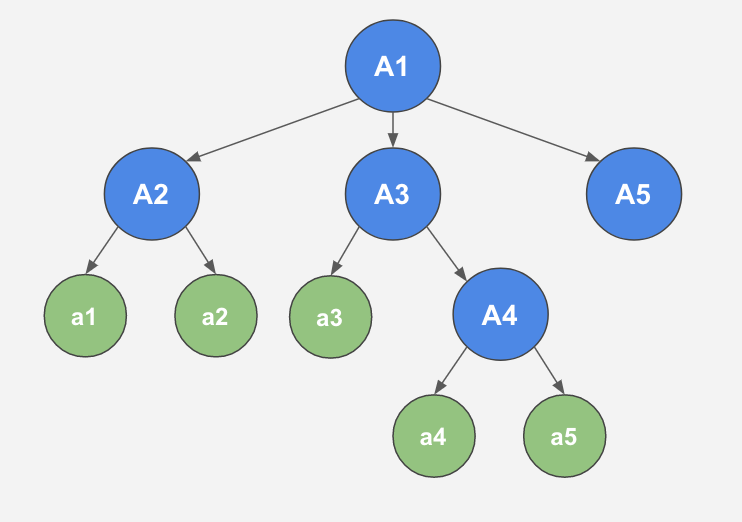
\includegraphics[width=11cm, height=8cm]{async-tree.png}
\vspace*{10px}

Every node has child nodes as their arguments. So, \cit{a1}, \cit{a2}, \cit{a3}, \cit{a4}, \cit{a5}, \cit{A5} are \textit{leaves} of the tree and they are being called first at the same time. When their results are received, their parents will be ready to be invoked (\cit{a1}, \cit{a2}, \cit{a3}, \cit{a4}, \cit{a5} are already ready in that case, so we just add them to the arguments of their parent).

\cit{A1} is a root of the tree, so we invoke it last. \cit{A2} never waits for the results of \cit{A3} or \cit{A4}, because \cit{A2} just does not need them. But \cit{A3} waits for the result of \cit{A4}, and \cit{A1} waits for the results of \cit{A2}, \cit{A3} and \cit{A5}.

\newpage

So, the sequence of the calls would look like this:

\begin{lstlisting}
a1, a2, a3, a4, a5, A5 // at the same time
A2, A4 // at the same time
A3
A1
\end{lstlisting}

You might ask \textit{"What if I need to use the result that is represented by the \cit{A1}, how can I do that?"}. Well, it's very simple: you just wrap it with another async object that processes representation of the \cit{A1}.

\subsection{Program implementation}

For implementation Aync Tree Pattern we need following classes(abstractions): \cit{AsyncObject}, \cit{AsyncTree},
\cit{TreeNode}, \cit{SimpleTreeNode}, \cit{AsyncTreeNode}, \cit{NotDefinedAsyncTreeNode}, \cit{Event}, \cit{As} and \cit{NullError}.

\subsubsection{AsyncObject}

\cit{AsyncObject} has three types of methods: methods that must be(or can be) implemented by classes that extend it, methods that can be used in declarative composition and methods that are not allowed to be overridden(for internal usage). Also \cit{AsyncObject} has constructor.

\vspace*{10px}
\noindent
\textbf{Constructor}

\begin{lstlisting}

constructor(...args) {
  this.args = args;
  this.tree = new AsyncTree(this);
  this.next;
  this.cache = {};
  this.asKey;
}

\end{lstlisting}
\cit{...args} can be any type, including \cit{AsyncObject}. Every \cit{AsyncObject} encapsulates \cit{tree} that use it as a root field. Argument \cit{next} points to the next async tree if it set by \cit{after} method(by default it's undefined). Also every async object has \cit{cache} that is simple map. It's needed because cache must be visible in the global scope. Field \cit{asKey} is used as a key for saving representation(computing result) of the async object into the cache if method \cit{as} is invoked.

\vspace*{10px}

\subsubsection{Methods for implementing}

\begin{lstlisting}
definedAsyncCall() {
  throw new Error('asyncCall or syncCall must be defined');
}

definedSyncCall() {
  throw new Error('asyncCall or syncCall must be defined');
}

onError(error) {
  throw error;
}

onResult(result) {
  return result;
}

onErrorAndResult(error, result) {
  return error || result;
}

continueAfterFail() {
  return false;
}

callbackWithError() {
  return true;
}
\end{lstlisting}

Either of methods \cit{definedAsyncCall} or \cit{definedSyncCall} must be defined(implemented) in extended classes. If both of them are implemented then only \cit{definedAsyncCall} will be invoked. \cit{definedAsyncCall} is used for async calls, so it must return function of the async call. \cit{definedSyncCall} is used for synchronous processing, so it must return blocking function. The entire logic of using these methods will be shown in the \cit{AsyncTreeNode} class. 

Method \cit{onError} is used as a handler for errors that might happen in the async calls. And \cit{onResult} is used for post processing of the result of async/sync call.

If \cit{continueAfterResult} returns true, then \cit{onError} and \cit{onResult} will be ignored, and the represented result(or an error) of async object will be returned by \cit{onErrorAndResult}.

Method \cit{callbackWithError} must return \cit{true} if an error is expected in the callback of corresponding async call, otherwise it must return \cit{false}.

\vspace*{10px}

\subsubsection{Methods from public API}

\begin{lstlisting}

call() {
  this.propagateCache(this);
  this.tree.create().call();
}

after(asyncObject) {
  this.next = asyncObject;
  return this;
}

as(key) {
  this.asKey = key;
  return this;
}

\end{lstlisting}

Method \cit{call} is being invoked only of async object that is root of async tree. It propagates cache among all fields, so it will be able to access cache in every async object in the composition.

Method \cit{after} is used for setting next async tree that is being invoked after the current one and returns this async object. Obviously, this method can be used only for the root async object.

Method \cit{as} is used for setting \cit{key} for caching. It returns the async object with set \cit{key}.

\vspace*{10px}

\subsubsection{Internal methods (not for overriding)}

\begin{lstlisting}

iterateArgs(func) {
  this.args.forEach((arg, index) => {
    let isAsync = arg instanceof AsyncObject;
    let isEvent = arg instanceof Event;
    func(arg, index, isAsync, isEvent);
  });
}

hasNoArgs() {
  return this.args.length === 0;
}

readyToBeInvoked(readyResultsNum) {
  return this.args.length === readyResultsNum;
}

callNextTreeIfExists() {
  if (this.next) {
    this.propagateCache(this.next);
    new AsyncTree(this.next).create().call();
  }
}

propagateCache(arg) {
  if (arg instanceof AsyncObject) {
    arg.withCache(this.cache);
    arg.iterateArgs(
      arg => this.propagateCache(arg)
    );
  }
}

withCache(cache) {
  this.cache = cache;
  return this;
 }
 
saveValueIntoCacheIfNeeded(value) {
  if (this.asKey) {
    this.cache[this.asKey] = value;
  }
  return this;
}

\end{lstlisting}

Method \cit{iterateArgs} is a proxy method, which avoid using \textit{getters} and \textit{setters} for processing \cit{...args} of the async object.

Method \cit{hasNoArgs} checks if async object encapsulates anything.

Method \cit{readyToBeInvoked} compares number of ready results that are computed by child nodes(\cit{...args}) and number of all \cit{..args}. If they are equal, that means that we can compute result of this async object.

Method \cit{callNextTreeIfExists} is used for calling next async tree if it exists.


\end{document}
